\section{Introduction}
\textit{Ab initio} structure prediction algorithms typically start with a coarse grained search of conformational space through the assembly of previously picked structural fragments. As such, the accuracy of structure prediction is heavily dependent on the similarity of fragments to the target fold for each position \cite{Gront2011-ik}. Thus, the necessary structural information for accurate structure prediction must be encoded in the fragment library for a given target sequence. This approach allows the modelling of new protein folds by considering them as assemblies of already known building blocks, such as super-secondary structure motifs \cite{Fernandez-Fuentes2010-iu}. This idea is not novel and has been successfully applied in \gls{nmr} and X-ray crystallography studies \cite{Jones1986-kh,Delaglio2000-pu,Kontaxis2005-bz}. However, almost all implementations neglect target-specific information generally available to crystallographers through bioinformatics software. This information includes the primary sequence of the target, torsion angle predictions, predicted solvent accessibility or co-evolution information. In theory, all additional information should improve the generation of such fragment libraries by aiding the selection process or cross-validating the identified fragments.

Over the last decade, efforts have been made to improve the precision of structural fragment libraries used in \textit{ab initio} structure prediction \cite{Shen2013-ag,Li2008-fu,Kalev2011-te,Bhattacharya2016-bp,Wang2017-ox,De_Oliveira2015-ba,Gront2011-ik}. Various different algorithms have been developed to generate static and dynamic fragment libraries. Static fragment libraries are those pre-computed and generally consist of common super-secondary structure motifs. In comparison, dynamic fragment libraries consist of fragments of variable lengths acknowledging the fragment-dependent optimal length. Most commonly used in \textit{ab initio} structure prediction are dynamic algorithms, such as FLIB \cite{De_Oliveira2015-ba}, NNmake \cite{Gront2011-ik} or HHfrag \cite{Kalev2011-te}. Dynamic-library producing algorithms differ in their definition of ideal fragment lengths, the default number of fragments used per position and the way in which fragments are extracted. However, these algorithms typically share the same additional sequence-based information used to aid the selection of target fragments, which usually includes sequence similarity, three-state secondary structure prediction and torsion angle prediction.

Given that fragment libraries selected to perform \textit{ab initio} structure prediction can contain high quality fragments or super-secondary structure motifs, those fragments must sometimes be suitable as \gls{mr} search models. Correct identification of true positives should allow for dynamic fragment selection to achieve \gls{mr} structure solution without the overhead of \textit{ab initio} structure prediction. Furthermore, dynamic algorithms could pick fragments of varying lengths, possibly matching co-evolution data or other externally obtainable restraints to validate fragments prior to any \gls{mr} attempt. As such, the work in this chapter focuses on exploring this idea using FLIB \cite{De_Oliveira2015-ba}, a dynamic fragment picking algorithm considering co-evolution data to verify fragments during the picking process.

\section{Methods}
\subsection{Target selection}
Four targets were manually selected for this study. The crystallographic data needed a resolution of around 1.5A with a single molecule in the asymmetric unit. The target chain length needed to be below 150 residues, and the fold of the protein structure to be either mixed \textalpha-\textbeta or all-\textbeta. A further target selection criterion was the availability of precise contact information for fragment selection.

The \gls{pdb} identifiers of the selected targets are: 1aba, 1lo7, 1u06, and 5nfc. The former two are described in \cref{table:methods_dataset_flume}. Target 1u06 is a recently published structure of \textalpha-spectrin SH3 domain (\gls{pdb} ID: 1kjl in \cref{table:methods_dataset_flume}) with a resolution of 1.49\AA. Target 5nfc is a recently published structure of Galectin-3 (\gls{pdb} ID: 1kjl in \cref{table:methods_dataset_flume}) with a resolution of 1.59\AA. This resulted in a dataset with similar attributes for each target: crystallographic data resolution of $~1.5$\AA\ with a single molecule in the asymmetric unit, and the target chain length of $<150$ residues. Each fold class, mixed \textalpha-\textbeta and all-\textbeta, contained two targets.

\subsection{Fragment picking using FLIB}
FLIB \cite{De_Oliveira2015-ba} requires four inputs: the predicted secondary structure, predicted torsion angles, residue-residue contact pair data and a copy of the \gls{pdb}. The secondary structure for each target was predicted using PSIPRED v4.0 \cite{Jones1999-fi} with default parameters. The torsion angles were predicted using SPIDER2 \cite{Heffernan2015-wp} with default parameters, and residue-residue contact pairs using METAPSICOV v1.04 \cite{Jones2015-wp} with default parameters. HHBLITS v2.0.16 \cite{Remmert2011-ze} with database version \texttt{uniprot20\_2016\_02} was used by METAPSICOV to generate the \gls{msa} for contact prediction of each target sequence. BLASTP v2.2.31+ \cite{Altschul1990-nc,Camacho2009-ue} was used by PSIPRED with the UNIPROT database version \texttt{uniref90-2016\_06}. The local copy of the \gls{pdb} for fragment picking was downloaded on August 11, 2016.

Two modifications were made to the default FLIB v1.01 (\url{https://github.com/sauloho/FLIB-Coevo}) protocol. The first focuses on exclusion of fragments with $>90$\% helical content (assigned by DSSP \cite{Frishman1995-ns}). If fragments with $>90$\% helical content are allowed and residues are predicted to be part of an \textalpha-helix, fragment libraries tend to be overpopulated for these positions with short helices. This would generate fragment libraries similar to ideal helix libraries, which is not the purpose of this work. The second modification was to allow fragments with \gls{rmsd} $>10.0$\AA\ to the reference structure to be considered. This modification to the FLIB algorithm was implemented for development purposes by the authors to validate the performance of the algorithm. However, to allow for the automatic calculation of \gls{rmsd} value of each fragment without deliberately excluding less-similar fragments this modification was lifted.

Two-hundred fragments were picked per target sequence position. Top-$L$ or $L/2$ contact pairs were selected from both METAPSICOV STAGE 1 and STAGE 2 predictions with a minimum sequence separation of either 6 or 12 residues. Helical fragments were either included or excluded. The fragment length ranged from either 6 or 12 (dependent on minimum sequence separation) to 63 residues. Overall, this generated 16 fragment libraries per target.

Each fragment library was then filtered to remove homologs of the target to be solved. BLASTP and HHPRED \cite{Soding2005-sx} searches were conducted to identify homologous PDB entries. The BLASTP search was performed identically to \textcite{De_Oliveira2015-ba} using an E-value cutoff of 0.05. The HHPRED search parameters were identical to the MPI-Toolkit \cite{Biegert2006-ny} webserver version (\url{https://toolkit.tuebingen.mpg.de/}). Fragments derived from PDB entries identified by BLASTP and HHPRED (probability score of $\geq20.0$) were excluded from the fragment libraries.

All per-target fragments were then binned by their peptide lengths. Subsequently, they were ranked by FLIB scores and \gls{rmsd} values, and the best fragment from each length-dependent bin selected. Partially redundant fragments of the same template structure consisting of the same region with varying flanking residues were kept, if they were ranked top for each fragment length group. Finally, the coordinates of the fragment backbone atoms were extracted to create poly-Alanine search models.

Note, the FLIB score refers in this chapter to the predicted torsion angle score for a given fragment, which FLIB uses in its default routine to rank fragments with lower scores being more favourable \cite{De_Oliveira2015-ba}. 

\subsection{Molecular Replacement in MRBUMP}
The previously extracted fragments were subjected to the \gls{mr} pipeline MRBUMP \cite{Keegan2008-hk}. This uses PHASER \cite{McCoy2007-bf} for \gls{mr}, REFMAC5 \cite{Murshudov2011-we} for refinement and SHELXE \cite{Thorn2013-ir} for density modification and main-chain tracing. MRBUMP default parameters were used with exception of the PHASER \gls{rmsd} estimate. Each fragment was subjected to MRBUMP using PHASER \gls{rmsd} values of 0.1, 0.6 and 1.0\AA.

\subsection{Assessment of FLIB fragments}
Fragment torsion angles --- predicted by SPIDER2 \cite{Heffernan2015-wp} --- were assessed using the \gls{mae}, which evaluates the average absolute difference between the predicted and experimentally determined angles \cite{Heffernan2015-wp}. To account for the periodicity of an angle, the smaller value of the absolute difference $d_i$ and $360-d_i$ was used. The coverage of a fragment library was assessed by the proportion of residues present in at least one fragment in the library. The precision of a fragment library was defined by the fraction of \gls{tp} fragments. All fragments with an \gls{rmsd} of $<1.5$\AA\ were considered \gls{tp} else \gls{fp}. The equation used to calculated the precision score is \cref{eq:methods_precision}. The \gls{rmsd} value, as calculated by FLIB \cite{De_Oliveira2015-ba}, was computed between the aligned residues of the corresponding crystal structure and the fragment. \Gls{mr} success for each search model was solely assessed by SHELXE scores, whereby a \gls{cc} score of $\geq25.0$ combined with an \gls{acl} score of $\geq10.0$ was required.

\section{Results}
In this study, the main objective was to determine if peptide fragments derived from protein structures in the \gls{pdb} could be reliably selected and trialed in \gls{mr} to achieve structure solutions. The fragment picking algorithm FLIB \cite{De_Oliveira2015-ba} was used to pick fragments given its novel approach of validating selected fragments against a set of predicted residue-residue contacts.

\subsection{Precision of FLIB input data}
The FLIB algorithm requires two sets of input data --- the predicted secondary structure and per-residue torsion angles --- for each target sequence alongside an optional third source of information in form of co-evolution data. The first part of the analysis in this study focuses on these data given that the FLIB fragment picking heavily relies on the individual features in the selection and scoring of each individual fragment \cite{De_Oliveira2015-ba}. Poor data at this stage could lead to poor fragments that would be unsuitable for \gls{mr} trials given that high accuracy, i.e. a low \gls{rmsd} value between the search model and target, is required.

The secondary structure prediction highlighted high precision between each target's prediction and the DSSP-assigned \cite{Frishman1995-ns} secondary structure of the target reference structure (\cref{fig:ample_flib_psipred}). The three targets with \gls{pdb} identifiers 1aba, 1lo7 and 1u06 have secondary structure predictions with a precision of $>89$\%. The fourth target, 5nfc, shows comparatively poor precision of 50.7\% over all residues in the PSIPRED prediction and the DSSP assignment using the reference crystal structure. However, 11 out of 13 secondary structure features are correctly predicted, suggesting successful fragment picking is possible.

\begin{figure}[H]
	\centering
	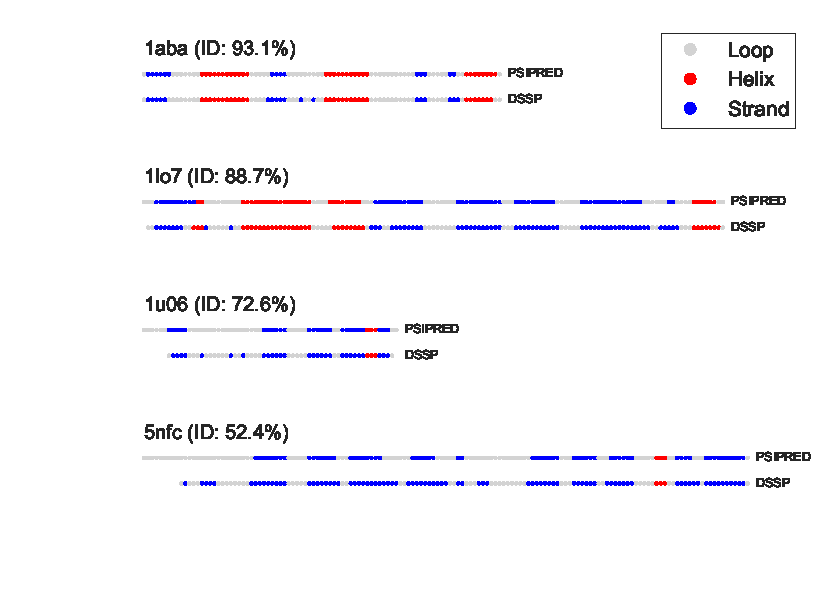
\includegraphics[width=\textwidth]{ample_flib_psipred.pdf}
	\caption[PSIPRED schema for FLIB targets]{Schematic comparison of PSIPRED \cite{Jones1999-fi} secondary structure prediction and DSSP \cite{Frishman1995-ns} assignment. Percentage identity is provided next to each identifier. The identity was computing using the Hamming distance over all positions present in the target sequence and reference structure.}
	\label{fig:ample_flib_psipred}
\end{figure}

The contact prediction data for METAPSICOV STAGE 1 and STAGE 2 predictions demonstrate the high precision scores achievable by this algorithm (\cref{table:ample_flib_contact_precision}). In this study, the top contact pairs at cutoffs $L$ and $L/2$ were provided to the FLIB algorithm. All targets have precision scores for both sets of predictions at both cutoff levels of $>0.6$ (\cref{table:ample_flib_contact_precision}). A comparison of the sets of contact pairs shows that only every third (for $L/2$ contacts) or every other (for $L$ contacts) contact pair is shared between both METAPSICOV STAGE predictions highlighting the importance of trialling both when selecting FLIB fragments (Jaccard index in \cref{table:ample_flib_contact_precision}).

\begin{table}[H]
  \centering
  \caption[Contact prediction summary for FLIB targets]{Precision scores for METAPSICOV \cite{Jones2015-wp} STAGE 1 and STAGE 2 contact predictions. Jaccard index calculated for the same $L$-dependent selection of contact pairs between METAPSICOV STAGE 1 and STAGE 2 predictions.}
  \label{table:ample_flib_contact_precision}
  \begin{tabularx}{\textwidth}{X X X X X X X}
      \hline
	  \multirow{2}{*}{\textbf{Target}} & \multicolumn{3}{c}{\textbf{$L/2$ contact pairs}} & \multicolumn{3}{c}{\textbf{$L$ contact pairs}} 	\\ \cline{2-7}
	  							&  	Prec\textsubscript{STAGE 1}	& 	Prec\textsubscript{STAGE 2}	& 	Jaccard 	& 	Prec\textsubscript{STAGE 1} 	& 	Prec\textsubscript{STAGE 2} 	& 	Jaccard	\\
	  \hline
	  1aba						&	0.884	&	0.884	&	0.303	&	0.713	&	0.759	&	0.513		\\
	  1lo7						&	0.857	&	0.957	&	0.308	&	0.738	&	0.837	&	0.446		\\
	  1u06						&	0.839	&	0.806	&	0.378	&	0.710	&	0.787	&	0.459		\\
	  5nfc						&	0.822	&	0.836	&	0.327	&	0.619	&	0.762	&	0.434		\\ 
	  \hline
  \end{tabularx}
\end{table}

Given the two METAPSICOV contact prediction files, both show localised clusters of contact pairs characteristic for secondary structure features (\cref{fig:ample_flib_cmaps}). These clusters are more populated with contact pairs in METAPSICOV STAGE 2 predictions. This behaviour is to-be-expected given that the second stage in METAPSICOV screens the first to remove singleton contact pairs whilst enriching the already existing clusters \cite{Jones2015-wp}. Besides the visual analysis, a cluster determination study on each of those contact maps further confirmed a higher singleton frequency in METAPSICOV STAGE 1 predictions. The latter contain on average 9\% more singleton contact pairs, and thus a higher degree of noise.

\begin{figure}[H]
	\centering
	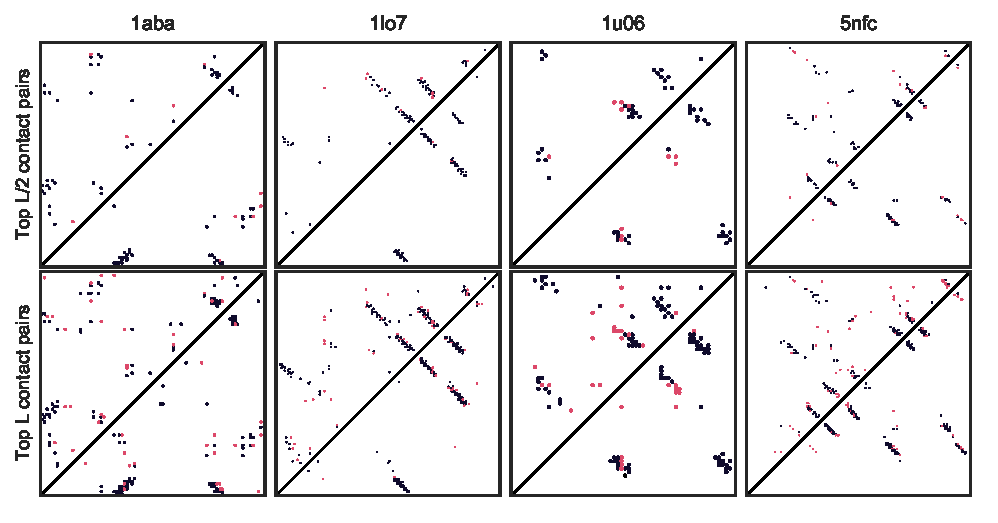
\includegraphics[width=\textwidth]{ample_flib_cmaps.pdf}
	\caption[Contact map comparison for FLIB targets]{Comparison of $L/2$ and $L$ correctly and incorrectly predicted contact pairs for four FLIB targets. Contacts were predicted using METAPSICOV \cite{Jones2015-wp} STAGE 1 (top left) and STAGE 2 (bottom right). True and false positive contact pairs were identified using a 8\AA\ cutoff between C\textalpha\ (C\textbeta\ in case of GLY) atoms of a reference crystal structure. PSIPRED \cite{Jones1999-fi} secondary structure prediction provided along the diagonal.}
	\label{fig:ample_flib_cmaps}
\end{figure}

An analysis of the \gls{mae} of torsion angles between the SPIDER2 \cite{Heffernan2015-wp} prediction and a corresponding reference crystal structure highlights accurate predictions for three of four targets (\cref{fig:ample_flib_spider2}). The largest \gls{mae}\textsubscript{\textphi} across the four target sequences is $24.347^{\circ}$, and the largest \gls{mae}\textsubscript{\textpsi} is $45.459^{\circ}$ (\gls{mae} values for \gls{pdb} entry 1u06). The smallest \gls{mae}\textsubscript{\textphi} is $13.822^{\circ}$ (\gls{pdb} ID: 1aba) and smallest \gls{mae}\textsubscript{\textpsi} is $17.273^{\circ}$ (\gls{pdb} ID: 1lo7). Segments in sequence space with regular secondary structure, as predicted by PSIPRED \cite{Jones1999-fi}, result primarily in low \gls{mae} values of torsion angles. In contrast, unstructured regions highlight much larger \gls{mae} values indicating the difficulty of predicting these regions. Noticeably, the \gls{mae}\textsubscript{\textpsi} appears to be much larger in those regions than the \gls{mae}\textsubscript{\textphi} for the same residue.

In summary, all target sequences have FLIB input data of good quality, which should allow FLIB to select fragments of suitable accuracy for \gls{mr}.

\begin{figure}[H]
	\centering
	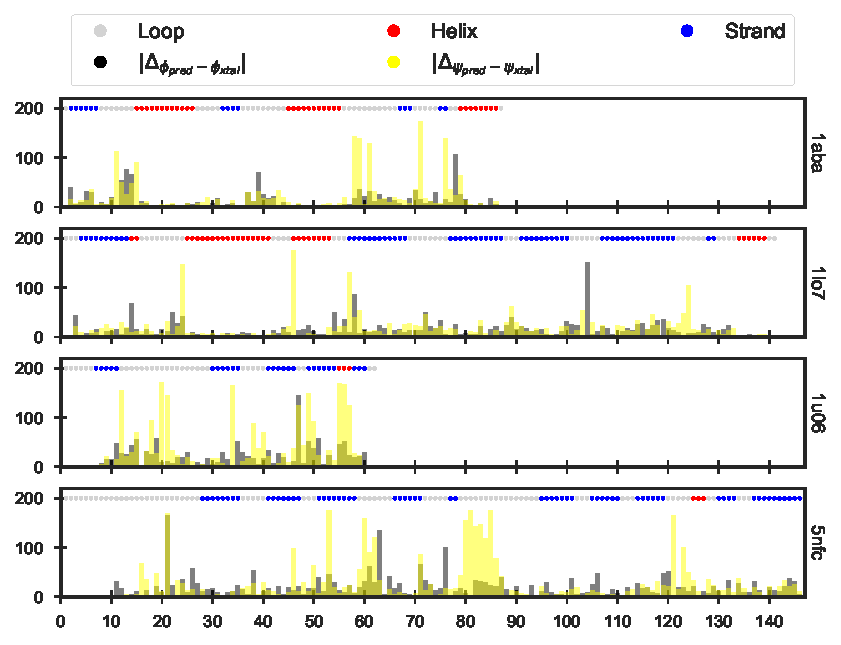
\includegraphics[width=\textwidth]{ample_flib_spider2.pdf}
	\caption[SPIDER2 torsion angle prediction analysis of FLIB targets]{Comparison of \gls{mae} of torsion angles predicted by SPIDER2 and extracted from a corresponding \gls{pdb} structure. PSIPRED \cite{Jones1999-fi} secondary structure prediction provided alongside the \gls{mae} values.}
	\label{fig:ample_flib_spider2}
\end{figure}

\subsection{FLIB fragment picking}
Sixteen FLIB fragment libraries were picked for each protein target in this study. Each fragment library consisted of one permutation of one of two contact prediction files and altering input parameters.

Across all four targets, the FLIB algorithm selected a total of 8,535,458 fragments (\cref{table:ample_flib_frag_summary}). The fragment libraries show similar statistics across the four protein targets despite the diversity in fold and chain lengths. The mean FLIB score is ~3,200 score units with a mean \gls{rmsd} of 9.00\AA. Fragments for the alpha-spectrin SH3 domain (\gls{pdb} ID: 1u06) scored the lowest mean FLIB score with 3,034 units; however, the same target scored the worst by mean \gls{rmsd} with an average of 9.47\AA. In contrast, fragments picked for the sequence of the bacteriophage T4 glutaredoxin (\gls{pdb} ID: 1aba) achieved the best mean \gls{rmsd} of 7.85\AA\ given the second highest mean FLIB score of 3,217 units (\cref{table:ample_flib_frag_summary}).

\begin{table}[H]
  \centering
  \scriptsize
  \caption[FLIB fragment characterics across four protein targets]{Summary of fragment statistics for FLIB libraries selected for four protein targets. Count\textsubscript{H} corresponds to the count of fragments extracted from homologs.}
  \label{table:ample_flib_frag_summary}
  \begin{tabularx}{\textwidth}{X X X X X X X X X}
      \hline
      \multirow{2}{*}{\textbf{Target}} & \multirow{2}{*}{\textbf{Count}} & \multirow{2}{*}{\textbf{Count\textsubscript{H}}} & \multicolumn{3}{c}{\textbf{FLIB score}} & \multicolumn{3}{c}{\textbf{\gls{rmsd}}} \\ \cline{4-9}
      		&			&			& Median 	& Mean 		& Std Dev 	& Median 	& Mean 	& Std Dev \\
      \hline
      1aba	& 2,091,321	& 45,133		& 3,061	& 3,217	& 1,405	& 7.70	& 7.85	& 3.81	\\
	  1lo7	& 2,497,813	& 23,396		& 3,187	& 3,371	& 1,497	& 9.00	& 9.43	& 4.61	\\
      1u06	& 1,133,517	& 60,159		& 2,901	& 3,034	& 1,306	& 9.51	& 9.47	& 3.94	\\
      5nfc	& 2,812,807	& 48,828		& 2,982	& 3,127	& 1,316	& 8.89	& 9.16	& 4.18	\\
      \hline
      Total	& 8,535,458	& 177,516		& 3,049	& 3,208	& 1,397	& 8.68	& 8.96	& 4.25	\\
      \hline
  \end{tabularx}
\end{table}

A split of the per-target fragment libraries by input options highlights the better fragment library quality under certain conditions with regards to the mean FLIB score and \gls{rmsd} (\cref{fig:ample_flib_flibcond}). In particular, top-$L$ (6 residues sequence separation) METAPSICOV STAGE 1 contact predictions yielded the lowest for both metrics across all targets. A comparison of the sequence separation, i.e. using all contact pairs or medium- and long-range ones only, strongly suggests much lower and thus more favourable scores for using short-, medium- and long-range contact pairs. A very similar difference is noticeable for METAPSICOV STAGE 2 contact predictions (\cref{fig:ample_flib_flibcond}). 

\begin{figure}[H]
	\centering
	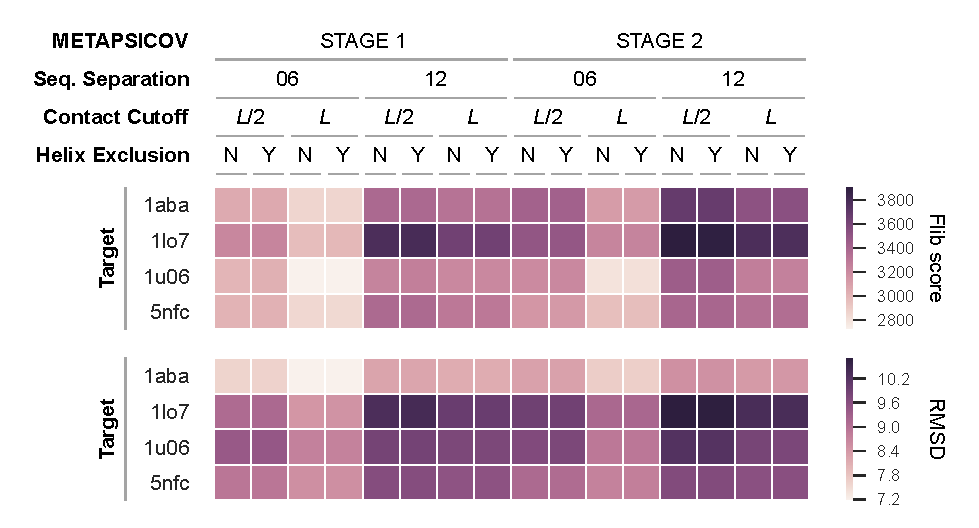
\includegraphics[width=\textwidth]{ample_flib_flibcond.pdf}
	\caption[FLIB fragment library comparison]{FLIB fragment library comparison for four targets highlighting the differences in mean FLIB score and \gls{rmsd} by starting with different subsets of contact predictions. $L$ refers to the number of residues per target sequence. $Y$ refers to idealised \textalpha-helical fragment exclusion during fragment picking; $N$ refers to treating those fragments like all others.}
	\label{fig:ample_flib_flibcond}
\end{figure}

An analysis of the coverage of the target sequence with respect to each picking strategy further demonstrates the benefits of starting with METAPSICOV STAGE 1, i.e. noisier contact predictions (\cref{fig:ample_flib_fragtps}). Coverage is more evenly spread across the target sequences compared to missing regions especially for target 4-hydroxybenzoyl CoA thioesterase (\gls{pdb} ID: 1lo7) when starting with METAPSICOV STAGE 2 predictions. Noticeably, none of the picking strategies yielded any fragments for the C-termini of \textalpha-spectrin SH3 domain (\gls{pdb} ID: 1u06) and galectin-3 CRD (\gls{pdb} ID: 5nfc) (\cref{fig:ample_flib_fragtps}). Furthermore, an analysis of the precision of fragments in each library strongly supports the benefits of starting with top-$L$ (6 residues sequence separation) METAPSICOV STAGE 1 contact pairs. Across all four targets, the coverage of correct fragments (classed by \gls{rmsd} $<1.5$\AA\ to the reference structure) is highest for this condition. This is of particular importance for \textalpha-spectrin SH3 domain (\gls{pdb} ID: 1u06) and galectin-3 CRD (\gls{pdb} ID: 5nfc), for which most strategies picked very few to no correct fragments. Excluding idealised \textalpha-helical fragments does not affect the quality of the FLIB libraries greatly. A consideration of differences in mean FLIB and \gls{rmsd} scores shows \textDelta\ differences of 25.68 and 0.06 between the comparable libraries, i.e. with and without idealised \textalpha-helical fragments.

\begin{figure}[H]
	\centering
	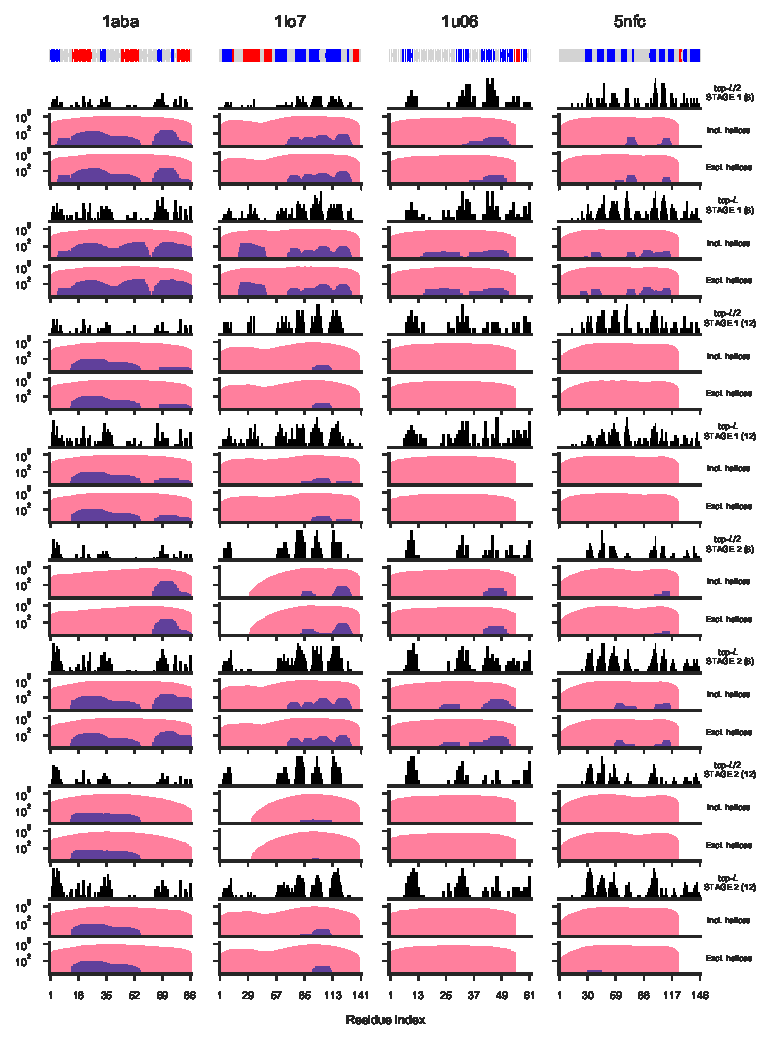
\includegraphics[width=\textwidth]{ample_flib_fragtps.pdf}
	\caption[Coverage and precision of Flib fragment libraries]{Summary of the coverage and precision of FLIB fragment libraries according to their target sequence. The coverage of all fragments with respect to their target-aligned sequence register are shown in red bars, and fragments with \gls{rmsd} $<1.5$\AA\ to the reference structure in blue. The predicted secondary structure of each target sequence is given at the top: \textalpha-helices (red), \textbeta-strands (blue), and loops (gray). Contact prediction information is illustrated using black bars. The fragment frequency is shown using a log-scale.}
	\label{fig:ample_flib_fragtps}
\end{figure}

Given that FLIB uses co-evolution data to help select fragments, it is little surprise that higher degrees of \gls{tp} fragments co-localise with high-density contact pair regions along the target sequence (\cref{fig:ample_flib_fragtps}). This characteristic explains less \gls{tp} fragments in top-$L/2$ fragment libraries because less contacts (compared to top-$L$) are available during fragment selection. The resulting selection is purely based on the FLIB score which might not yield high-accuracy fragments (\gls{rmsd} $<1$\AA) as frequently. Therefore, the co-localisation of \gls{tp} FLIB fragments and regions of high-density contact predictions highlights the importance of adding this additional source of information to pick fragments. 

\subsection{FLIB fragment selection for Molecular Replacement}
One of the most important aspects of bypassing \textit{ab initio} structure prediction and using the relevant fragments directly as \gls{mr} search models is the selection of the fragments with the highest similarity between fragment and target structure.

A fragment's FLIB score --- its predicted torsion angle score --- has the highest correlation with the \gls{rmsd} of a fragment compared to all other scores used in the FLIB protocol \cite{De_Oliveira2015-ba}. To validate this finding, all non-homologous fragments in this study were tested for a correlation between a their FLIB scores and \gls{rmsd} values. The Spearman's rank-order correlation coefficient analysis confirms the correlation between a fragment's FLIB and \gls{rmsd} scores (\cref{fig:ample_flib_flibspearman}). However, the strength of the correlation varies greatly between different fragment libraries and targets. The optimal fragment picking strategy --- top-$L$ (6 residues sequence separation) METAPSICOV STAGE 1 --- results in the strongest correlations across all targets. The same contact pair selection with METAPSICOV STAGE 2 predictions results in the second greatest correlations. Noticeably, the bacteriophage T4 glutaredoxin (\gls{pdb} ID: 1aba) fragment libraries show much more positive correlations than the remaining targets. The fragments selected for \textalpha-spectrin SH3 domain (\gls{pdb} ID: 1u06) show the overall weakest correlations.

\begin{figure}[H]
	\centering
	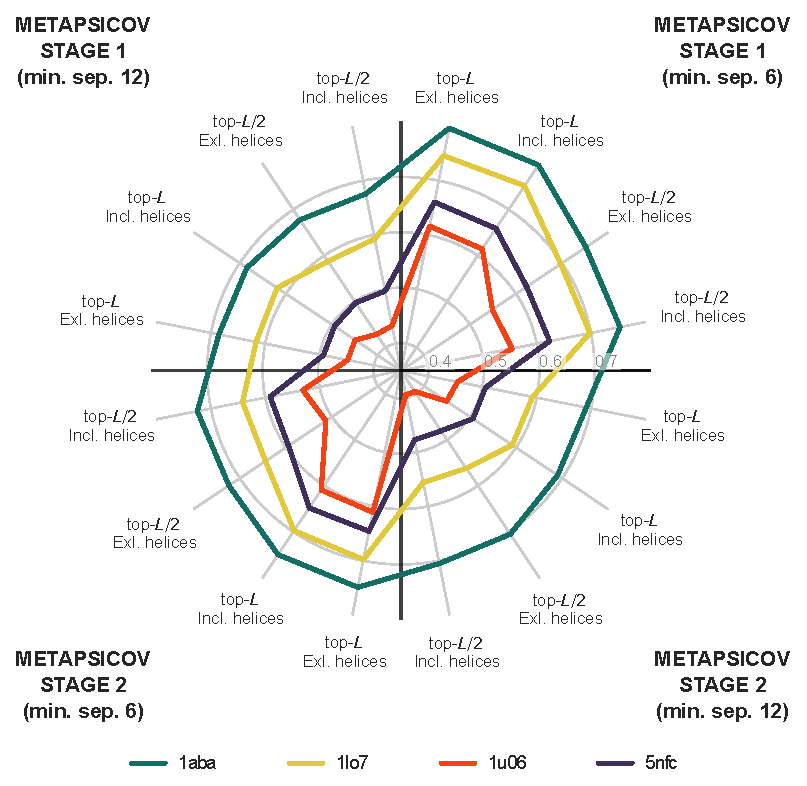
\includegraphics[width=\textwidth]{ample_flib_flibspearman.pdf}
	\caption[Spearman rank-order correlation coefficient analysis of FLIB fragments]{Spearman rank-order correlation coefficient analysis of FLIB fragments given the 16 unique fragment picking strategies across four targets. P-values of all Spearman correlations are $<0.001$ and not shown for simplicity of the plot.}
	\label{fig:ample_flib_flibspearman}
\end{figure}

Further inspection of the fragments and the relationship between each fragment's FLIB score and \gls{rmsd} value reveals a small subset of outliers in each fragment library. These fragments (hereafter referred to as outlier fragments) are sparse in each library with an overall mean count of $<0.2$\%. An analysis for unique characteristics of these outliers, which would allow for their exclusion, reveals no unique feature. These fragments contain all secondary structure types, span the entire target sequence and range over all peptide lengths. Furthermore, they occur in all fragment libraries, irrelevant of their original picking strategy. The only characteristic setting these outlier fragments apart from the remaining set is a \gls{rmsd} value of $>30$\AA. Nevertheless, it appears that these outlier fragments with unusually high \gls{rmsd} values are never included in the final fragment search model set, given that their overall FLIB\textsubscript{min} score is 796 units (one order of magnitude more than the overall minimum for the remaining fragments).

An analysis of the fragment metrics in the final \gls{mr} set (6,547 fragments) further supports the positively linear relationship between a fragment's FLIB score and \gls{rmsd} (\cref{fig:ample_flib_finalrelat}). Furthermore, the size of the fragments also positively correlates with the the FLIB ($\rho_{Spearman}=0.860$, $p<0.001$) and \gls{rmsd} ($\rho_{Spearman}=0.697$, $p<0.001$) values. Longer fragments with higher dissimilarity with respect to the target show higher FLIB scores and \gls{rmsd} values (\cref{fig:ample_flib_finalrelat}). Notably, a cluster of large fragments with some of the highest FLIB scores in the set show a reasonable similarity to their target structure (\cref{fig:ample_flib_finalrelat}). All fragments in this cluster were picked for the bacteriophage T4 glutaredoxin sequence (\gls{pdb} ID: 1aba) and extracted from the same region of the crystal structure of the actin-related protein ARP8 (\gls{pdb} ID: 4am6). In comparison, some smaller fragments with peptide lengths $<50$ residues and lower FLIB scores of $<3000$ show the highest \gls{rmsd} values in the final set.

\begin{figure}[H]
	\centering
	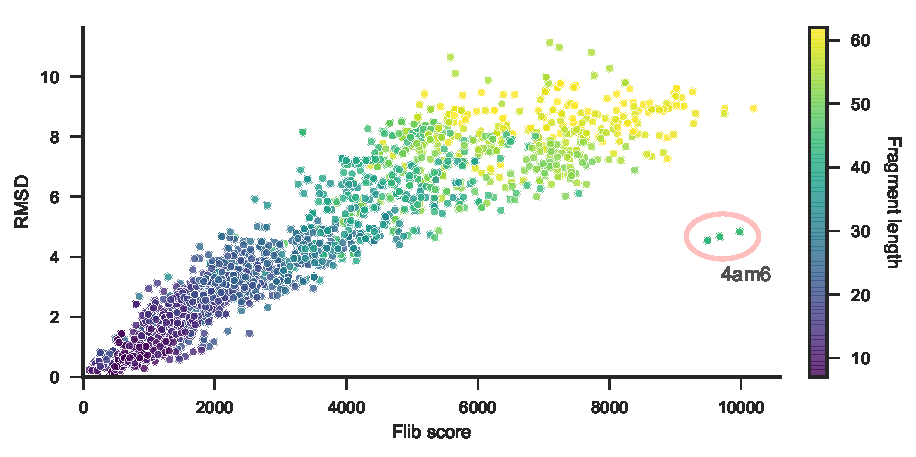
\includegraphics[width=\textwidth]{ample_flib_finalrelat.pdf}
	\caption[Correlation analysis for final FLIB \gls{mr} fragments]{Scatterplot highlighting the positive correlation between fragment FLIB scores and \gls{rmsd} values. The plot contains all fragments independent of target or picking strategy. The colour of each scatter point illustrates the fragment length. All extreme outlier fragments are highlighted with their \gls{pdb} identifiers as labels. The shaded area indicates a 54\% of fragments that follow a near-perfect positive correlation ($\rho_{Spearman}=0.947$, $p<0.001$).}
	\label{fig:ample_flib_finalrelat}
\end{figure}

One further unique aspect of this study compared to other fragment-\gls{mr} approaches is the use of residue-residue contact information to select fragments during picking, preferring those which satisfy at least one contact pair (Saulo de Oliveira, personal communication). In the final set 39\% of all fragments satisfy at least one, 26\% at least two and 20\% at least three contact pairs. Across the four targets, 50\% of all fragments selected for 4-hydroxybenzoyl CoA thioesterase (\gls{pdb} ID: 1lo7) satisfy at least one predicted contact pair (\cref{fig:ample_flib_consatis}). In comparison, 28\% of fragments selected for the \textalpha-spectrin SH3 domain (\gls{pdb} ID: 1u06) satisfy at least one contact pair.

\begin{figure}[H]
	\centering
	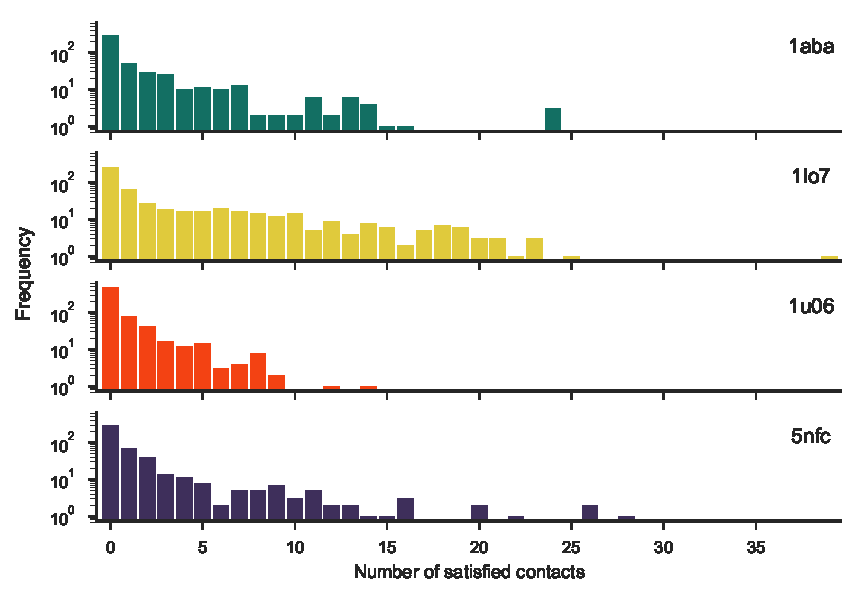
\includegraphics[width=\textwidth]{ample_flib_consatis.pdf}
	\caption[Distribution of contact precision for FLIB fragments]{Distribution of contact precision for FLIB fragments selected as \gls{mr} search models separated on a per-target basis.}
	\label{fig:ample_flib_consatis}
\end{figure}

Thus, the final set of FLIB fragment \gls{mr} search models spans a wide range of peptide lengths, \gls{rmsd} values, contact precision scores, and generally secondary structure make-up. To illustrate the latter, a random selection of sample fragments is illustrated in \cref{fig:ample_flib_search_models}. Importantly, not a single super-secondary structure motif dominates the set, increasing the sampling diversity to be undertaken during \gls{mr}.

\begin{figure}[H]
	\centering
	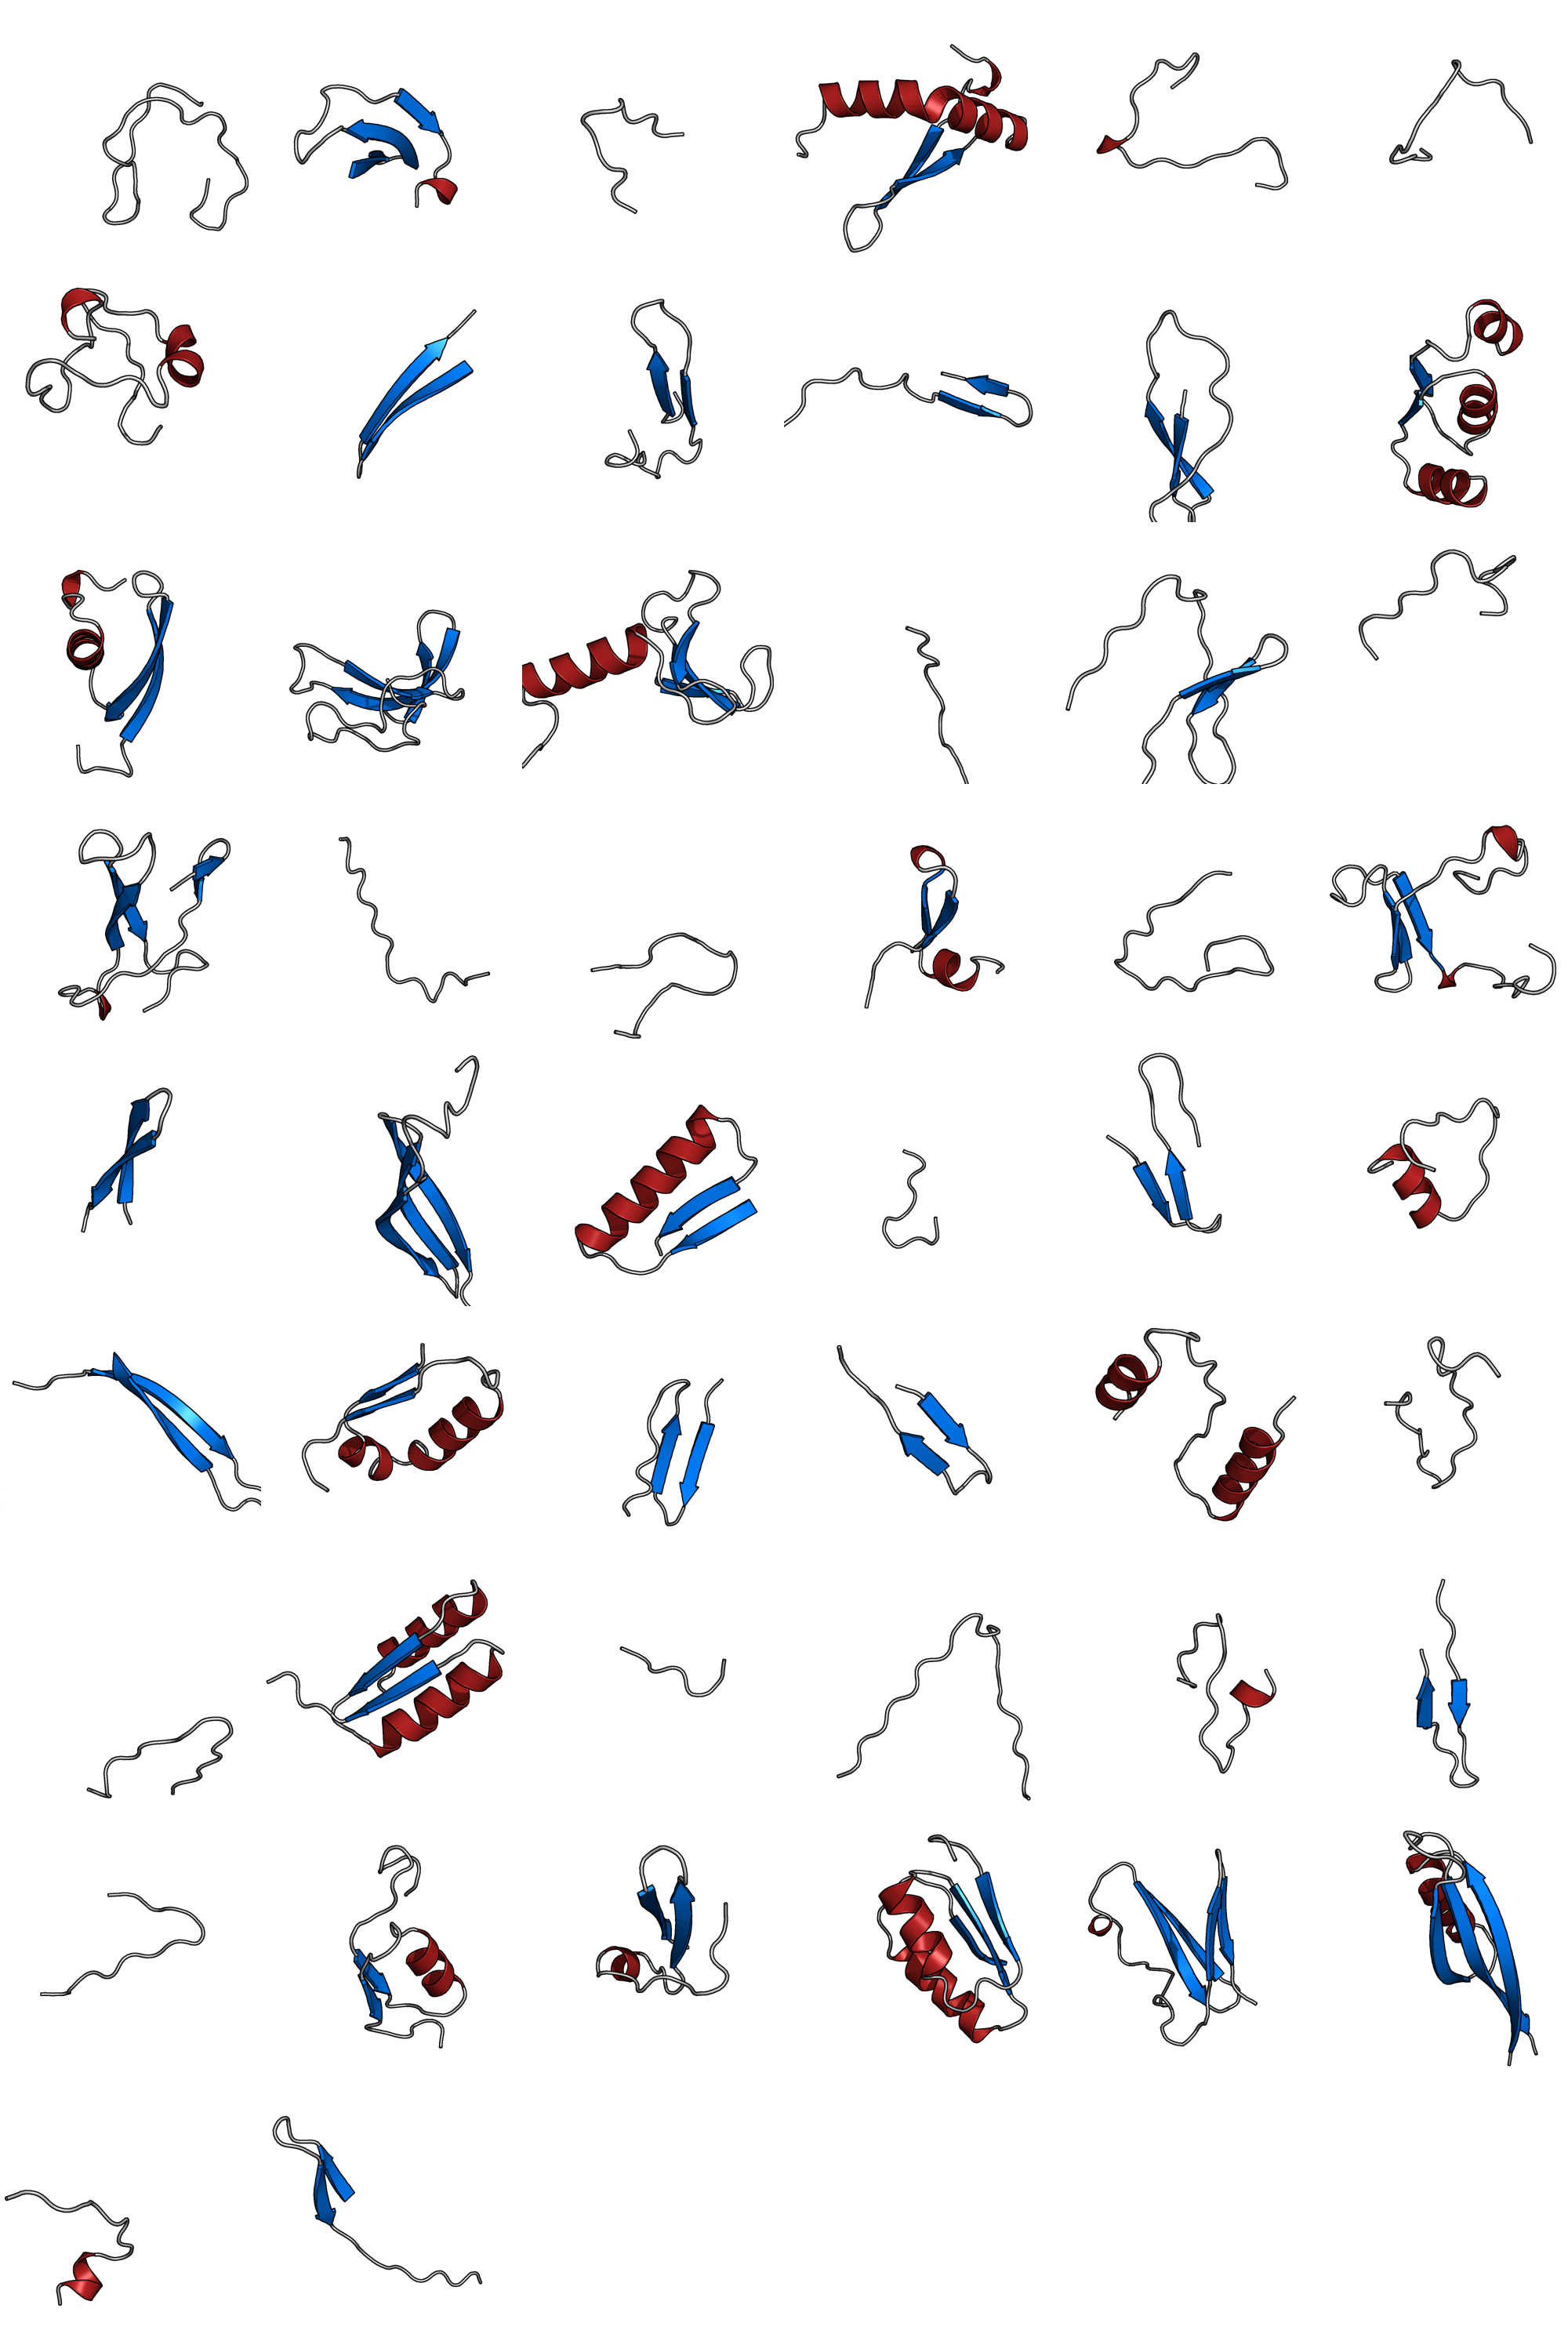
\includegraphics[width=\textwidth]{ample_flib_search_models2.png}
	\caption[Fragment search models derived from FLIB]{Non-redundant sample of FLIB fragment search models selected for four different protein targets. Secondary structure defined by and visualisation done in PyMOL \cite{Schrodinger_LLC2015-jz}. Unpaired \textbeta-strands rendered using the loop style.}
	\label{fig:ample_flib_search_models}
\end{figure}

\subsection{Molecular Replacement using FLIB fragments}
FLIB fragments picked for four target sequences using a variety of FLIB input options generated $>6,500$ fragments, which were subjected to the \gls{mr} pipeline MRBUMP with their corresponding target experimental data. Given that each fragment was trialled with three different PHASER \gls{rmsd} values, a total of 19,716 \gls{mr} attempts were made across four target structures. Out of nearly 20,000 \gls{mr} attempts, 299 led to the structure solutions of two targets, namely the T4 glutaredoxin (\gls{pdb} ID: 1aba) and \textalpha-spectrin SH3 domain (\gls{pdb} ID: 1u06) (\cref{fig:ample_flib_mrsummary}).

\begin{figure}[H]
	\centering
	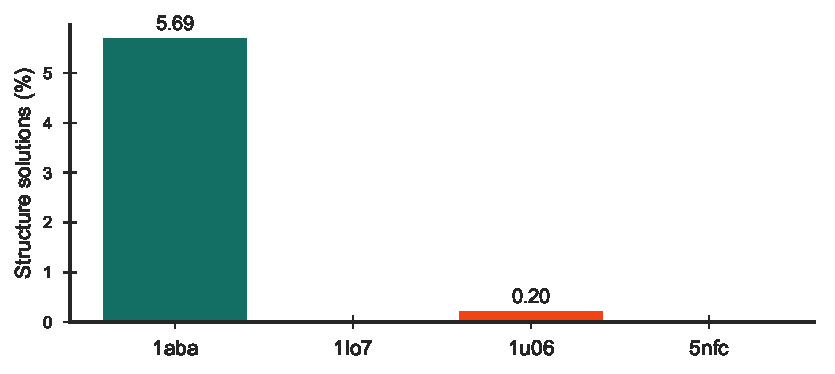
\includegraphics[width=\textwidth]{ample_flib_mrsummary.pdf}
	\caption[MR structure solutions by FLIB target]{Distribution of structure solutions by FLIB target. All \gls{mr} attempts total to 19,716, out of which 299 are structure solutions. Values above each bar indicates percentage search models successful out of the corresponding set.}
	\label{fig:ample_flib_mrsummary}
\end{figure}

The total of 299 \gls{mr} structure solutions were achieved by 70 sequence-unique fragments. Sixty-nine of those fragments were picked from 60 unique structures for the T4 glutaredoxin (\gls{pdb} ID: 1aba) leading to 97\% of all structure solutions. In comparison, a single fragment, selected from three different fragment libraries, led to 9 structure solutions of the \textalpha-spectrin SH3 domain (\gls{pdb} ID: 1u06). The largest FLIB fragment leading to a structure solution contained 37 residues and the smallest 10.

A division of FLIB-fragment search models by their respective origin libraries provides strong evidence that METAPSICOV STAGE 1 contact predictions allows for the selection of the most accurate fragments (\cref{fig:ample_flib_flibcond}), which directly translates into the structure solution count (\cref{fig:ample_flib_flibcondmr}). Furthermore, this division also highlights and supports the quality of fragment libraries picked with top-$L$ (6 residues sequence separation) METAPSICOV STAGE 1 predictions. Trialling the optimal fragment picking strategy with and without helical fragments ($>90$\% \textalpha-helical content assigned using DSSP) resulted in the library without outperforming the other (\cref{fig:ample_flib_flibcondmr}, 3\textsuperscript{rd} and 4\textsuperscript{th} bars). 

\begin{figure}[H]
	\centering
	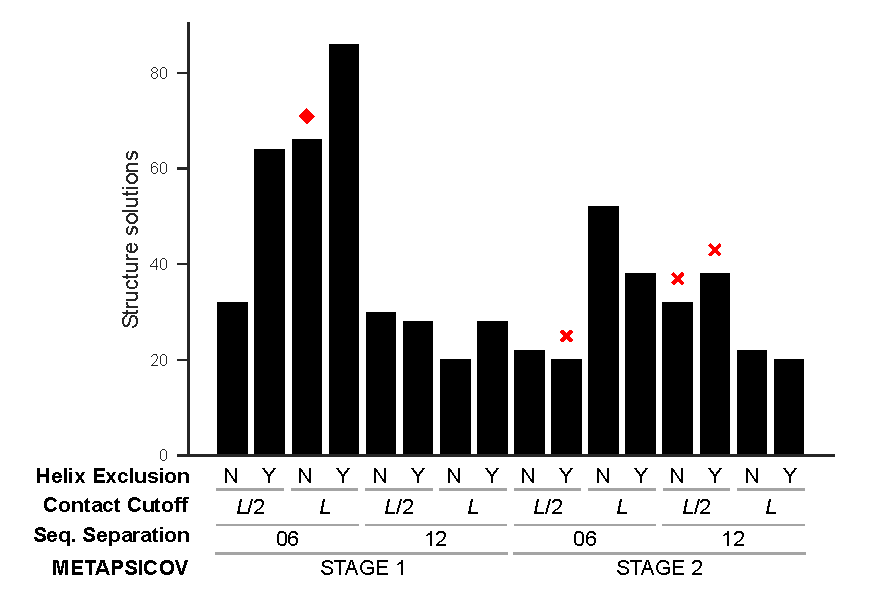
\includegraphics[width=\textwidth]{ample_flib_flibcondmr.pdf}
	\caption[MR structure solutions by FLIB library]{Distribution of structure solutions by FLIB library configuration. The optimal fragment picking strategy, as assessed by FLIB values, is highlighted with a red diamond to illustrate that the method that picks the best fragments is close to, but not the absolute best for ultimate structure solution. Fragment picking strategies leading to solutions of \textalpha-spectrin SH3 domain (\gls{pdb} ID: 1u06) are highlighted with red crosses.}
	\label{fig:ample_flib_flibcondmr}
\end{figure}

An analysis of the binned results by fragment-ranking or PHASER \gls{rmsd} value confirms the expected outcome: the top fragments selected by fragment \gls{rmsd} score result in more structure solutions than their FLIB score counterparts (\cref{fig:ample_flib_mrbyconfig}). To reiterate, all FLIB fragments were grouped by their peptide length, and the top fragment in each group selected when sorted by either FLIB or \gls{rmsd} values. When separating the total number of structure solutions by the score that made each fragment the best in its original library, it becomes clear that two-thirds of solutions were achieved with fragments scoring best by \gls{rmsd}. However, the structure of \textalpha-spectrin SH3 domain (\gls{pdb} ID: 1u06) was only solved with fragments that scored best in their FLIB fragment libraries by FLIB score. Furthermore, a separation of attempts by PHASER input \gls{rmsd} value suggests a value of 0.1 to be the most favourable.

\begin{figure}[H]
	\centering
	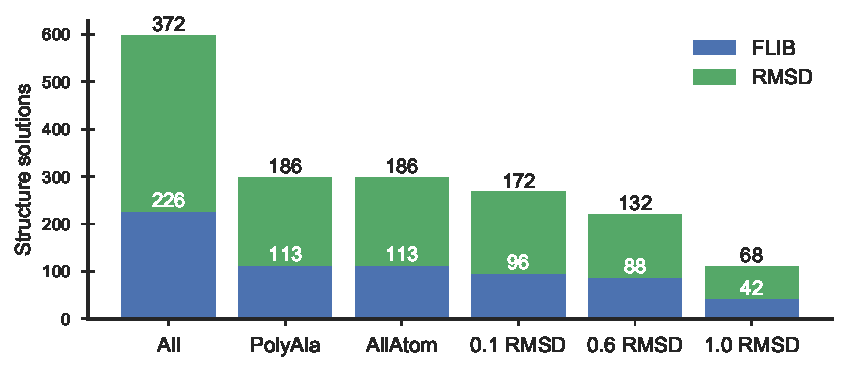
\includegraphics[width=\textwidth]{ample_flib_mrbyconfig.pdf}
	\caption[MR structure solutions by input parameters]{Distribution of structure solutions by fragment and MRBUMP configuration. The structure solution count is provided above each bar.}
	\label{fig:ample_flib_mrbyconfig}
\end{figure}

In \gls{mr}, the correct placement of very small structural fragment may not always be detectable by the output metrics of underlying software. In benchmarking exercises, the \gls{rio} metric has shown to be a very useful and powerful metric to detect such situations \cite{Thomas2015-ag,Simkovic2016-jx,Thomas2017-lq}. Given that the peptide lengths of FLIB fragments in this study range from 6 to 63 residues, the \gls{rio} score is most suitable in validating the correct placement of FLIB-fragment search models. Indeed, all fragments with SHELXE \gls{cc} $\geq25$ and \gls{acl} $\geq10$ contain at least 3 correctly placed C\textalpha\ atoms (i.e. a \gls{rio} score $\geq3$). Furthermore, the \gls{rio} metric indicates that more than 500 fragments have C\textalpha\ atoms placed within 1.5\AA\ of any atom in the target structure. However, only 4 residues are on average placed correctly, which was not enough to achieve structure solution (\cref{fig:ample_flib_mrrionorm}). All successful FLIB fragments have a minimum model- and target-normalised \gls{rio} scores of 29.7\% and 9.2\% (\cref{fig:ample_flib_mrrionorm}, green markers). 

\begin{figure}[H]
	\centering
	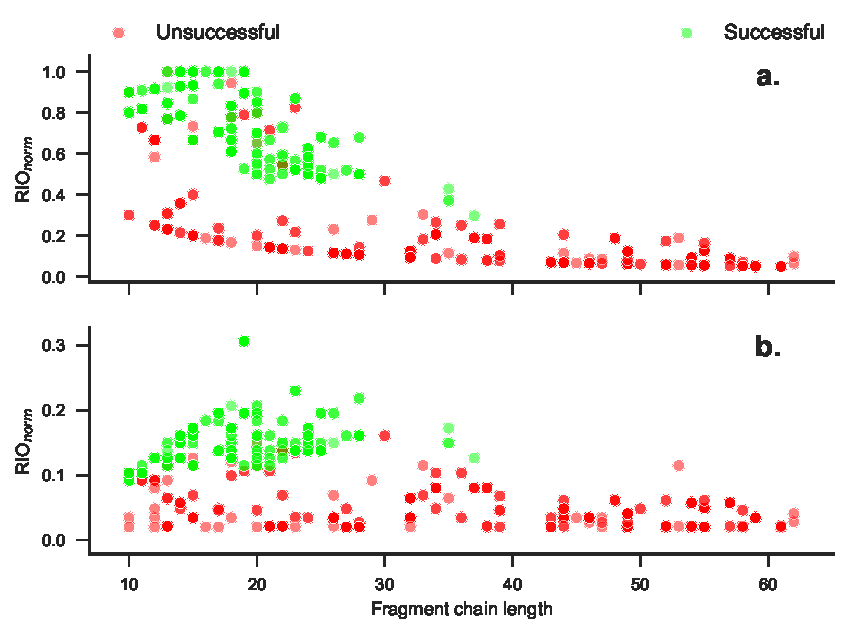
\includegraphics[width=\textwidth]{ample_flib_mrrionorm.pdf}
	\caption[Relationship between fragment chain length and normalised RIO scores.]{Dependence of normalised \acrlong{rio} (RIO\textsubscript{norm}) score on the fragment chain length. The two plots show  \gls{rio} scores normalised by the chain lengths of (a) the fragment and (b) the target. Colour coding indicates if the FLIB-fragment search model resulted in a structure solution. Each plot contains 890 fragment points; however, not all points are visible due to the superposition of individual scatter points because the same fragment was scored under different \gls{mr} conditions.}
	\label{fig:ample_flib_mrrionorm}
\end{figure}

In 33 \gls{mr} attempts more than 60\% of a fragment's residues were placed correctly, yet structure solution was not achieved. These trials affect exclusively fragments picked for the target sequences of T4 glutaredoxin (\gls{pdb} ID: 1aba) and 4-hydroxybenzoyl CoA thioesterase (\gls{pdb} ID: 1lo7). Overall, the 33 \gls{mr} attempts made were done with 17 fragments extracted from 15 templates containing between 10 and 23 amino acids. The fragments' \gls{rmsd} values range from 0.19 to 2.72\AA\ with a mean \gls{rmsd} of 1.10\AA. Surprisingly, almost all of these fragments contain primarily \textalpha-helices. Given the presence of helices in the fold of both targets (\cref{fig:ample_flib_psipred}) and the success of idealised fragments to solve such targets with data resolution $<2.0$\AA, it is a surprise to not see more structure solutions from these fragments.

Finally, the co-evolution data used in this study select fragments is a novelty in the field. Thus, it is of great interest to identify if fragments leading to structure solution satisfy many predicted residue-residue contacts. Eighty-seven percent ($n=61$) of all unique fragments leading to structure solutions for either target satisfy no predicted residue-residue contact. The remaining nine fragments, all of which lead to structure solutions of T4 glutaredoxin (\gls{pdb} ID: 1aba), satisfy either one ($n=4$), two ($n=4$) or 24 ($n=1$) predicted contacts. 

\begin{figure}[H]
	\centering
	\includegraphics[width=\textwidth]{ample_flib_mrchelatase.pdf}
	\caption[Example of FLIB fragment to MR solution]{Intermediary steps from donor structure to SHELXE main-chain autotrace for a fragment derived from cobalt chelatase found in \textit{Salmonella typhimurium} (\gls{pdb} ID: 1qgo). The structure solution was obtained against the target crystallographic data of T4 glutaredoxin (\gls{pdb} ID: 1aba). METAPSICOV STAGE 2 predicted contacts, against which the fragment was selected, are illustrated with \acrlong{tp} (green) and \acrlong{fp} (red) contacts (distance cutoff of 8\AA). 2mFo-DFc electron density maps shown at 2.0 sigma and radius around the peptide atoms of 5\AA. The \gls{rmsd} between the sequence-independently superposed structures of target and donor is 10.384\AA\ (computed with the \texttt{super} command in PyMOL \cite{Schrodinger_LLC2015-jz}).}
	\label{fig:ample_flib_mrchelatase}
\end{figure}

The fragment with 24 satisfied contacts is a particularly striking example of the value of the approach explored in this study (\cref{fig:ample_flib_mrchelatase}). The fragment was derived from the template structure of cobalt chelatase found in \textit{Salmonella typhimurium} (\gls{pdb} ID: 1qgo). The picked fragment contains 35 residues and its supersecondary structure consists of a two-strand \textbeta-sheet packing against a single \textalpha-helix. The majority of satisfied contact pairs are between C\textbeta\ atoms of the \textbeta-strands; however, a small number of individual contact pairs also identifies the packing of one \textbeta-strand against the \textalpha-helix (\cref{fig:ample_flib_mrchelatase}, top-right). Although not considered at this stage in the FLIB algorithm, this particular fragment satisfies 75\% of all relevant contact pairs. Most importantly though, this fragment was derived from an entirely unrelated protein structure, and thus illustrated the value in \textit{ab initio} structure prediction fragments as \gls{mr} search models.

\section{Discussion}
The main objective of this study was to investigate the application of FLIB structural fragments to \gls{mr}. Four experimental datasets were chosen and 16 FLIB fragment libraries built per target sequence varying primarily in the predicted residue-residue contact information. A selection of highest scoring fragments were then forwarded to MRBUMP to trial each fragment as \gls{mr} search model. The findings in this study validate the concept of this approach. Firstly, a positive correlation between a fragment's FLIB score and \gls{rmsd} value was identified. These correlations were target-independent and found, with various strengths, in all FLIB fragment libraries. Furthermore, this work has identified top-$L$ (6 residue sequence separation) METAPSICOV STAGE 1 contact pairs to be the optimal selection of contact pairs for the FLIB algorithm when starting with METAPSICOV predictions. The additional noise, typically filtered in the second STAGE of the METAPSICOV algorithm \cite{Jones2015-wp}, allowed for the selection of more accurate fragments across the entire target sequence. Lastly, trialling a selection of high-scoring FLIB fragments in routine \gls{mr} showed the usefulness of such fragments in attempting to solve protein structures. Two out of four targets were successfully solved albeit only trialling a small number of FLIB fragments per library.

Intuitively, most crystallographers would declare the limitations of this approach to be the size and quality of the selected FLIB fragments as well as the resolution of the crystallographic data. Although the former was long-thought to be a major limitation, more recent work highlighted the success of likelihood-based \gls{mr} methods (i.e., PHASER \cite{McCoy2007-bf}) with very small search models. \textcite{McCoy2017-wh} demonstrated the successful \textit{ab initio} \gls{mr} structure solution of aldose reductase starting from as little as two correctly placed atoms. Furthermore, automated \gls{mr} pipelines, such as AMPLE \cite{Bibby2012-vg} or the ARCIMBOLDO suite \cite{Millan2015-ih}, also successfully demonstrated \gls{mr} successes with search models comprising a fraction of the target structure. Thus, \gls{mr} structure solutions with FLIB fragments as short as 6 residues should not be considered impossible, although very challenging.

More importantly than size, \gls{mr} search models need to be sufficiently accurate to derive phase information for successful structure solution. The findings in this study highlight the success of identifying accurate fragments solely by the fragment's FLIB score. Given that the current FLIB implementation prefers a fragment if a single contact is satisfied, future research is required to identify the potential benefits of implementing the contact precision of a fragment in the overall FLIB score. In theory, higher precision scores should imply a closer match of the overall tertiary structure of the trialled region, and therefore this information needs to be considered as part of the overall score. Alternatively, selecting secondary structure motifs or substructures of templates by means of searching with a predicted contact map could be an attractive alternative. Recent studies indicated success in identifying sub-folds by means of \gls{cmo} \cite{Buchan2017-sy,Ovchinnikov2017-ma}.

However, FLIB fragments with near-identical subfolds to the target might not be traceable by current means of assessing structure solutions. Commonly, \gls{mr} success is judged by the combination of SHELXE \gls{cc} and \gls{acl} scores \cite{Thorn2013-ir}. However, it is known that \textbeta-strands are notoriously difficult to trace, and thus SHELXE might not pick up on correctly placed search models. Although this study did not suffer from this problem for fragments containing primarily \textbeta-strands, it did have correctly placed \textalpha-helices without structure solutions. Thus, future efforts need to be focused towards reliable assessments of correctly placed FLIB fragments.    

Finally, this work served primarily as proof-of-concept study, and thus attempted to explore a diversity of options. With a better understanding of input parameters future work could address a large-scale analysis of the suitability of these approaches. Furthermore, improvements to the FLIB algorithm originating from this work could help tailor the fragment picking process to obtain more closely matching fragments.
